% указываем класс документа
\documentclass[12pt,a4paper,openany]{extarticle}

% подключаем собственный стилевой файл 
\usepackage{mystyle}

% указываем язык (для автоматической вставки слов, типа "Глава", "Содержание", "Литература", "рис." и пр.
\selectlanguage{russian}

\begin{document}
\part*{Лабораторная работа №4\\
 Математическое описание модели на примере робота Segway}
\section{Методические рекомендации}
До начала работы студент должен выполнить предыдущие работы этого цикла. Необходимо знание основ теоретической механики и математических основ теории систем.
\section{Теоретические сведения}
В данной лабораторной работе предложен один из вариантов описания объекта управления. Полученая модель будет использоваться для расчета регулятора. Для начала остановимся на zOx плоскости, чтобы в~дальнейшем при расширении модели и введении дополнительных координат у нас был привычный базис.
Для начала мы будем использовать следующие обобщенные координаты:\\
$\theta$: среднее арифметическое значение углов поворота левого и правого колеса,\\
$\psi$: угол наклона робота оносительно вертикали.\\

\begin{figure}[H]
	\noindent\centering{
		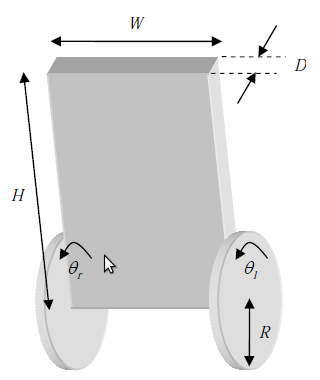
\includegraphics[scale=0.6]{Segway.png}
		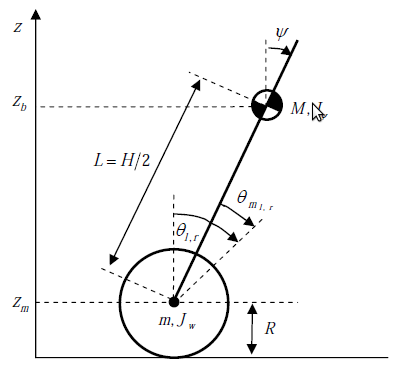
\includegraphics[scale=0.6]{Sheme.png}
	}
	\caption{Выбор системы координат.}
	\label{fig1}
\end{figure}


\begin{equation}
(x_m,\ z_m)=(\int\dot{x}_mdt,\ R),\ 
\dot{x}_mdt=R
\dot{\theta}.
\end{equation}

\begin{equation}
(x_b,\ z_b)=\left(x_m+L\sin\psi ,\ z_m+L\cos\psi \right)
\end{equation}

\begin{equation}
(x_b,\ z_b)=\left(\int R\dot{\theta} dt+L\sin\psi,\ R+L\cos\psi \right)
\end{equation}

Теперь выпишем уравнения поступательной кинетической энергии~$T_k$, вращательной кинетической энергии~$T_p$ и потенциальной энергии~$U$:

\begin{equation}
T_k=\cfrac12 M\left(\dot{x}_b^2+\dot{z}_b^2\right)\\
\end{equation}

\begin{equation}
T_p=\cfrac12J_\psi\dot{\psi}^2
\end{equation}

\begin{equation}
U=Mgz_b
\end{equation}

Если подставить значения соответствующих координат, то мы получим следущее выражение для кинетической энергии: $\cfrac12 M\left(\left(\left(\int R\dot{\theta}\ dt+L\sin\psi\right)'\right)^2
+((R+L\cos\psi)')^2 \right)$. 
Лагранжиан $\mathcal{L}$ будет выглядеть следующим образом:

\begin{equation}
\mathcal{L}=T_k+T_p-U
\end{equation}

Для автоматизации расчетов воспользуемся системой символьных вычислений Maxima и ее графической средой WxMaxima. Для упрощения ввода формул в Maxima, стоит заменить греческие буквы на английские. Введем полученное выражение в командную строку:

\begin{lstlisting}
V:expand(
	trigsimp(
		((diff(integrate(R*diff(O(t),t),t)+L*sin(y(t)),t))^2+
		(diff(R+L*cos(y(t)),t))^2)*M/2
		+J2*(diff(y(t),t))^2/2-M*g*(R+L*cos(y(t)))
	)
);
tex(V);
\end{lstlisting}

Команда \verb|trigsimp| используется для упрощения тригонометрических выражений, а \verb|expand| для раскрытия скобок. Команда \verb|tex| позволяет перевести полученный результат в tex-формат, что позволит вывести формулы в tex-документ или в виде рисунков.\\
После подстановки всех замен, котрые мы сделали, получаем следующее уравнение:

\begin{equation}
	 \mathcal{L}={{\dot\theta^2\,M\,R^2}\over{2}}+\dot\psi\,\dot\theta\,L\,M\,R\,\cos\psi-g\,
	  M\,R+{{\dot\psi^2\,L^2\,M}\over{2}}-g\,\cos \psi\,L\,M+{{\dot\psi^2\,{\it J_2}}\over{2}}
\end{equation} 

А уравнение Лагранжа запишем следующим образом:

\begin{equation}
\left\{  
	\begin{array}{rcl} 
	\cfrac{d}{dt}\cfrac{\partial \mathcal{L}}{\partial\dot{\theta}}-\cfrac{\partial \mathcal{L}}{\partial 			\theta}&=F_\theta\\
	\cfrac{d}{dt}\cfrac{\partial \mathcal{L}}{\partial\dot{\psi}}-\cfrac{\partial \mathcal{L}}{\partial \psi}&=F_\psi\\
	\end{array}   
	\right.
\end{equation}


Программа для Maxima будет следующей:

\begin{lstlisting}
expand(diff(diff(V,diff(O(t),t)),t)-diff(V,O(t)));
expand(diff(diff(V,diff(y(t),t)),t)-diff(V,y(t)));
\end{lstlisting}


Выполнив указанные дейсвия мы получим:

\begin{equation}
\left\{  
	\begin{array}{rcl}
	F_\theta&=&MR^2\ddot\theta+MRL\ddot\psi\cos\psi-MRL\dot\psi^2\sin\psi\\
	F_\psi&=&MRL\ddot\theta\cos\psi+(ML^2+J_\psi)\ddot\psi-MgL\sin\psi\\
	\end{array}   
	\right.
\end{equation}

Далее составим уравнения для двигателей нашего Segway:
\begin{equation}
(F_\theta,\ F_\psi)=\left(F_l+F_r,\ F_\psi\right)
\end{equation}

\begin{equation}
\left\{  
	\begin{array}{rcl}
	F_l&=&k_mI\\
	F_r&=&k_mI\\
	F_\psi&=&-2k_mI\\	
	\end{array}   
	\right.
\end{equation}

\begin{equation}
L_i\dot{I}=U+k_\omega(\dot\psi-\dot\theta)-R_\textit{я}I
\end{equation}
Так как индуктивность обмотки крайне мала, положим $L=0$:
\begin{equation}
I_{l,r}=\frac{U_{l,r}+k_\omega(\dot\psi-\dot\theta_{l,r})}{R_\textit{я}}
\end{equation}
Получим:
\begin{equation}
\left\{  
	\begin{array}{rcl}
	F_\theta&=&2\cfrac{k_m}{R_\textit{я}}U+2\cfrac{k_mk_\omega}{R_\textit{я}}(\dot\psi-\dot\theta)\\
	F_\psi&=&-2\cfrac{k_m}{R_\textit{я}}U-2\cfrac{k_mk_\omega}{R_\textit{я}}(\dot\psi-\dot\theta)\\	
	\end{array}   
	\right.
\end{equation}
Запишем окончательную систему уравнений, описывающих динамическую модель робота:
\begin{equation}
\left\{
\begin{array}{rcl}
	2\cfrac{k_m}{R_\textit{я}}U&=&MR^2\ddot\theta+MRL\ddot\psi\cos\psi-MRL\dot\psi^2\sin\psi+2\cfrac{k_mk_\omega}{R_\textit{я}}(\dot\psi-\dot\theta)\\
	-2\cfrac{k_m}{R_\textit{я}}U&=&MRL\ddot\theta\cos\psi+(ML^2+J_\psi)\ddot\psi-MgL\sin\psi-2\cfrac{k_mk_\omega}{R_\textit{я}}(\dot\psi-\dot\theta)\\	
	\end{array}   
	\right.
\end{equation}

Линеарезуем нашу модель. Для этого воспользуемся первым замечательным пределом $ \sin\psi=\psi $, а $ \cos\psi=1 $ при малых углах отклонения, до 15 градусов.

\begin{equation}
\left\{
\begin{array}{rcl}
	2\cfrac{k_m}{R_\textit{я}}U&=&MR^2\ddot\theta+MRL\ddot\psi-MRL\dot\psi^2\psi+2\cfrac{k_mk_\omega}{R_\textit{я}}(\dot\psi-\dot\theta)\\
	-2\cfrac{k_m}{R_\textit{я}}U&=&MRL\ddot\theta+(ML^2+J_\psi)\ddot\psi-MgL\psi-2\cfrac{k_mk_\omega}{R_\textit{я}}(\dot\psi-\dot\theta)\\	
	\end{array}   
	\right.
\end{equation}

Теперь нам необходимо избавиться от оставшихся нелинейностей, квадротов переменных и их произведений между собой. Мы пренебрегаем этими значениями только при условии, что угол отклонения от начального положения будет крайне мал.

\begin{equation}
\left\{
\begin{array}{rcl}
	2\cfrac{k_m}{R_\textit{я}}U&=&MR^2\ddot\theta+MRL\ddot\psi+2\cfrac{k_mk_\omega}{R_\textit{я}}(\dot\psi-\dot\theta)\\
	-2\cfrac{k_m}{R_\textit{я}}U&=&MRL\ddot\theta+(ML^2+J_\psi)\ddot\psi-2\cfrac{k_mk_\omega}{R_\textit{я}}(\dot\psi-\dot\theta)-MgL\psi\\	
	\end{array}   
	\right.
\end{equation}

Теперь мы получили систему уравнений, в которой с одной стороны мы имеем управляющее воздействие, а с другой линейные дифференциальные уравнения состояния объекта. В третьем уравнении содержится только одна переменная $\phi$ и ее производные. Поэтому мы будем рассматривать это уравнение отдельно от остальных. Введем вектора состояния $x^T=[\theta, \psi]$ и управления $u=U$, запишем первые два уравнения в матричной форме:

\begin{equation}
E\ddot{x}+F\dot{x}+Gx=Hu
\end{equation}

\begin{equation}
E=
\begin{bmatrix}
	MR^2&MRL\\
	MRL&ML^2+J_\psi\\
\end{bmatrix},
F=
\begin{bmatrix}
	2\cfrac{k_mk_\omega}{R_\textit{я}}&-2\cfrac{k_mk_\omega}{R_\textit{я}}\\
	-2\cfrac{k_mk_\omega}{R_\textit{я}}&2\cfrac{k_mk_\omega}{R_\textit{я}}\\
\end{bmatrix},
G=
\begin{bmatrix}
	0&0\\
	0&MgL\\
\end{bmatrix},
H=
\begin{bmatrix}
	2\cfrac{k_m}{R_\textit{я}}\\
	-2\cfrac{k_m}{R_\textit{я}}\\
\end{bmatrix}.
\end{equation}

Дальше запишем наше уравнение в следующей форме:

\begin{equation}
\ddot{x}=E^{-1}F\dot{x}+E^{-1}Gx+E^{-1}Hu
\end{equation}

Для того чтобы перейти к форме вход--состояние--выход, добавим к имеющемуся уравнению еще одно, $\dot\psi=\dot\psi$. Учитывая, что $E^{-1}G=\cfrac{1}{J_\psi}\begin{bmatrix} 0&M^2RL^2g\\0&M^2R^2Lg\\ \end{bmatrix}$, заменим вектор состояния на $x^T=[\psi, \dot\theta, \dot\psi]$:

\begin{equation}
\dot{x}=\begin{array}{|lcr|} 0&0&1\\ E^{-1}G[1,2]&&\\ E^{-1}G[2,2]&&E^{-1}F \end{array}x+\begin{array}{|lr|} 0&0\\ &E^{-1}H\end{array}u
\end{equation}

\section{Цель работы}
Получить нелинейную и линеаризованную модели объекта управления. Провести математическое моделирование переходных процессов в системе.

\section{Порядок выполнения работы}
\begin{enumerate}
	\item Вывод математической модели объекта управления.
	\begin{enumerate}
		\item Изобразите схематичный рисунок модели, обозначенной преподавателем.
		\item Выберите обобщенные координаты для описания объекта управления.
		\item Получите выражение для функции Лагранжа.
		\item Получите уравнения Лагранжа для каждой координаты.
		\item Линеарезуйте полученную модель.
	\end{enumerate}
	\item Математическое моделирование.
	\begin{enumerate}
		\item Постройте схему полученной математической модели, используя пакет прикладных математических программ для моделирования динамических систем.
		\item Осуществите моделирование системы.
	\end{enumerate}
	\item Обработка данных.
	\begin{enumerate}
		\item Выведите графики моделирования.
	\end{enumerate}
\end{enumerate}
\section{Содержание отчета}
\begin{enumerate}
	\item Вывод математической модели объкта.
	\item Описание объекта в~пространстве состояния.
	\item Схема моделирования и график, полученные при~математическом моделировании.
\end{enumerate}
\end{document}

\end{document}
